\chapter{Electron Ion Collider}\label{cha:EIC} % chktex 24

\section{Motivation...?}
just an introduction, further explanations of the processes in cha:physics

\section{Current Design Plan (from RHIC to EIC?)}

\begin{figure}[H]
    \centering
    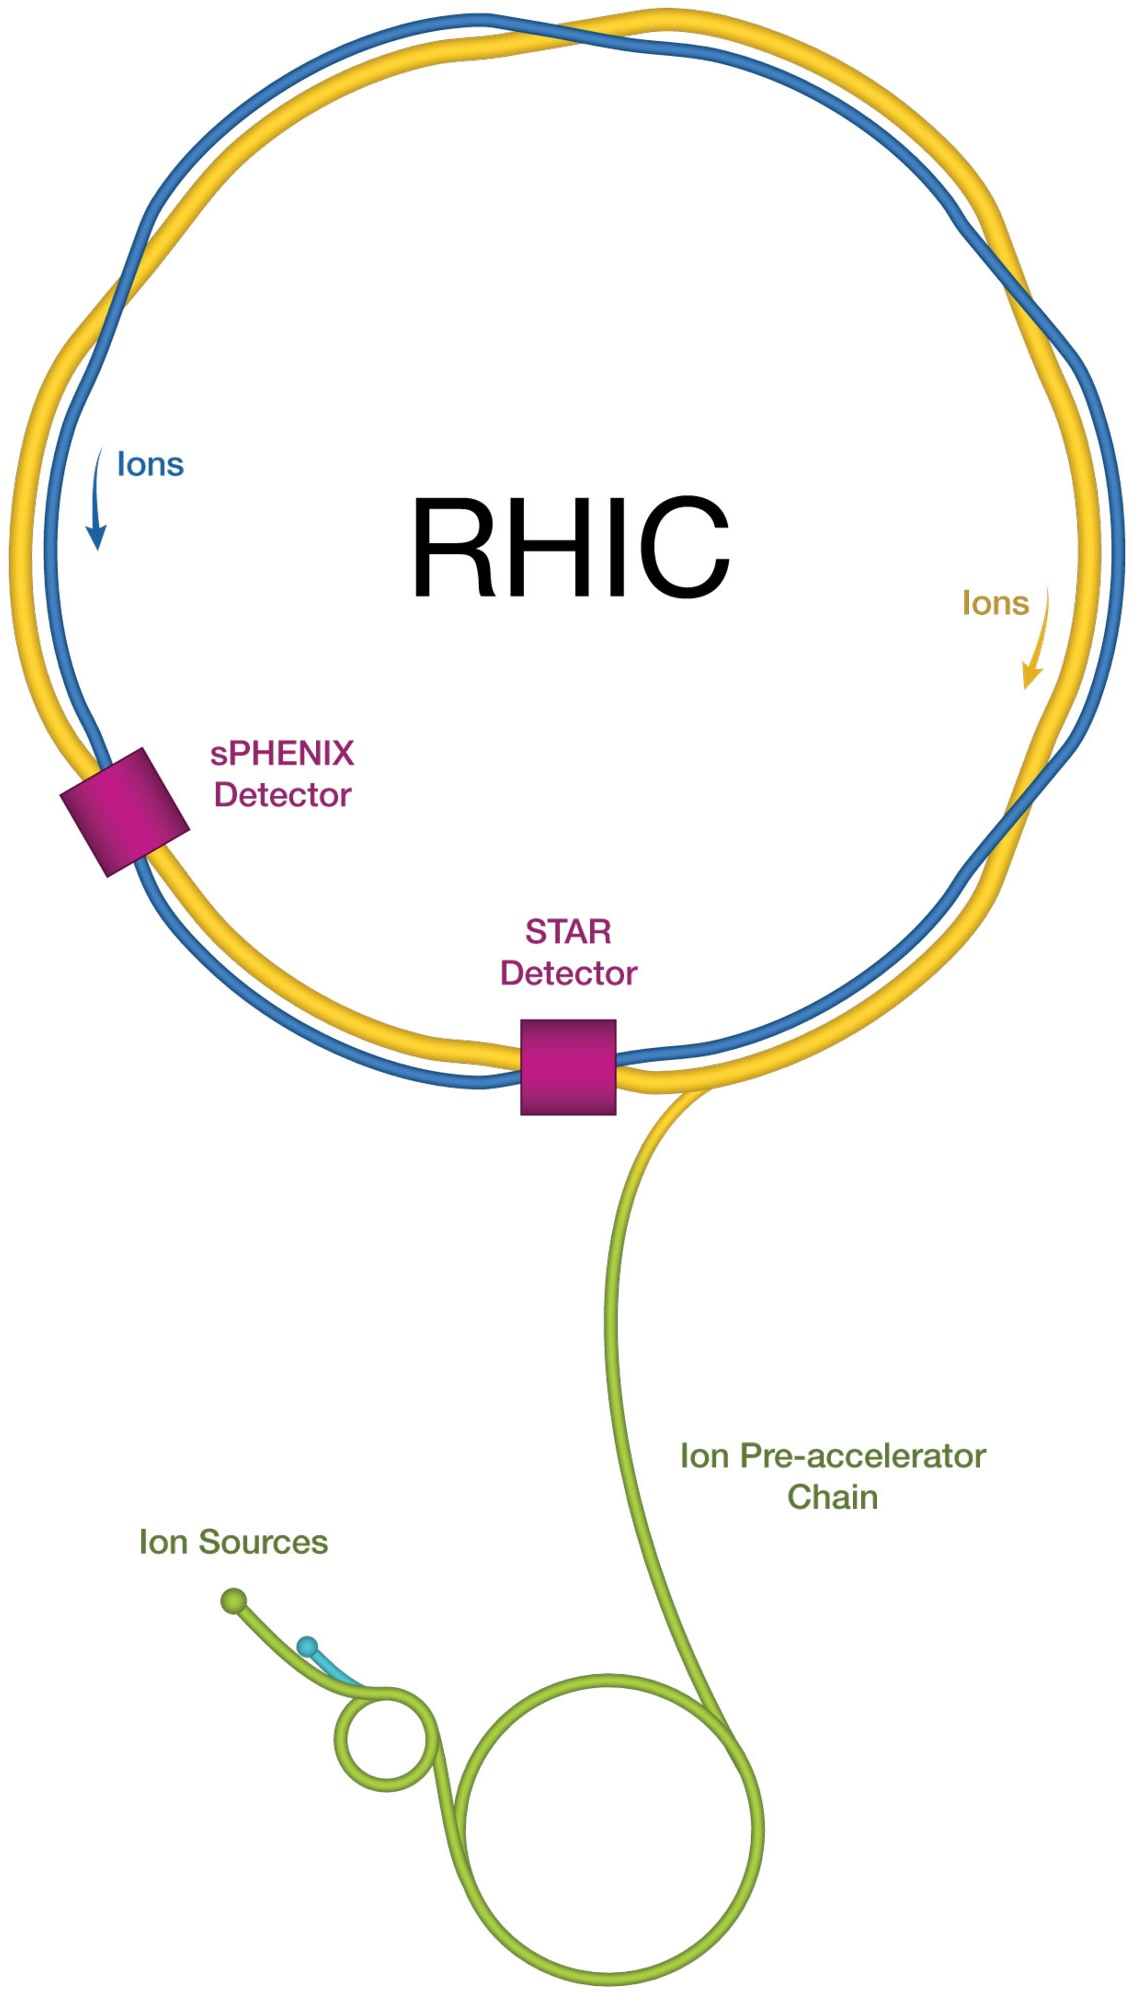
\includegraphics[width=.4\linewidth]{img/rhic.jpg}
    \caption{\url{https://www.flickr.com/photos/brookhavenlab/51980309345/in/album-72157714316624996}}
    \label{fig:eic:rhic}
\end{figure}
maybe next to each other? - EIC should be still larger?
\begin{figure}[H]
    \centering
    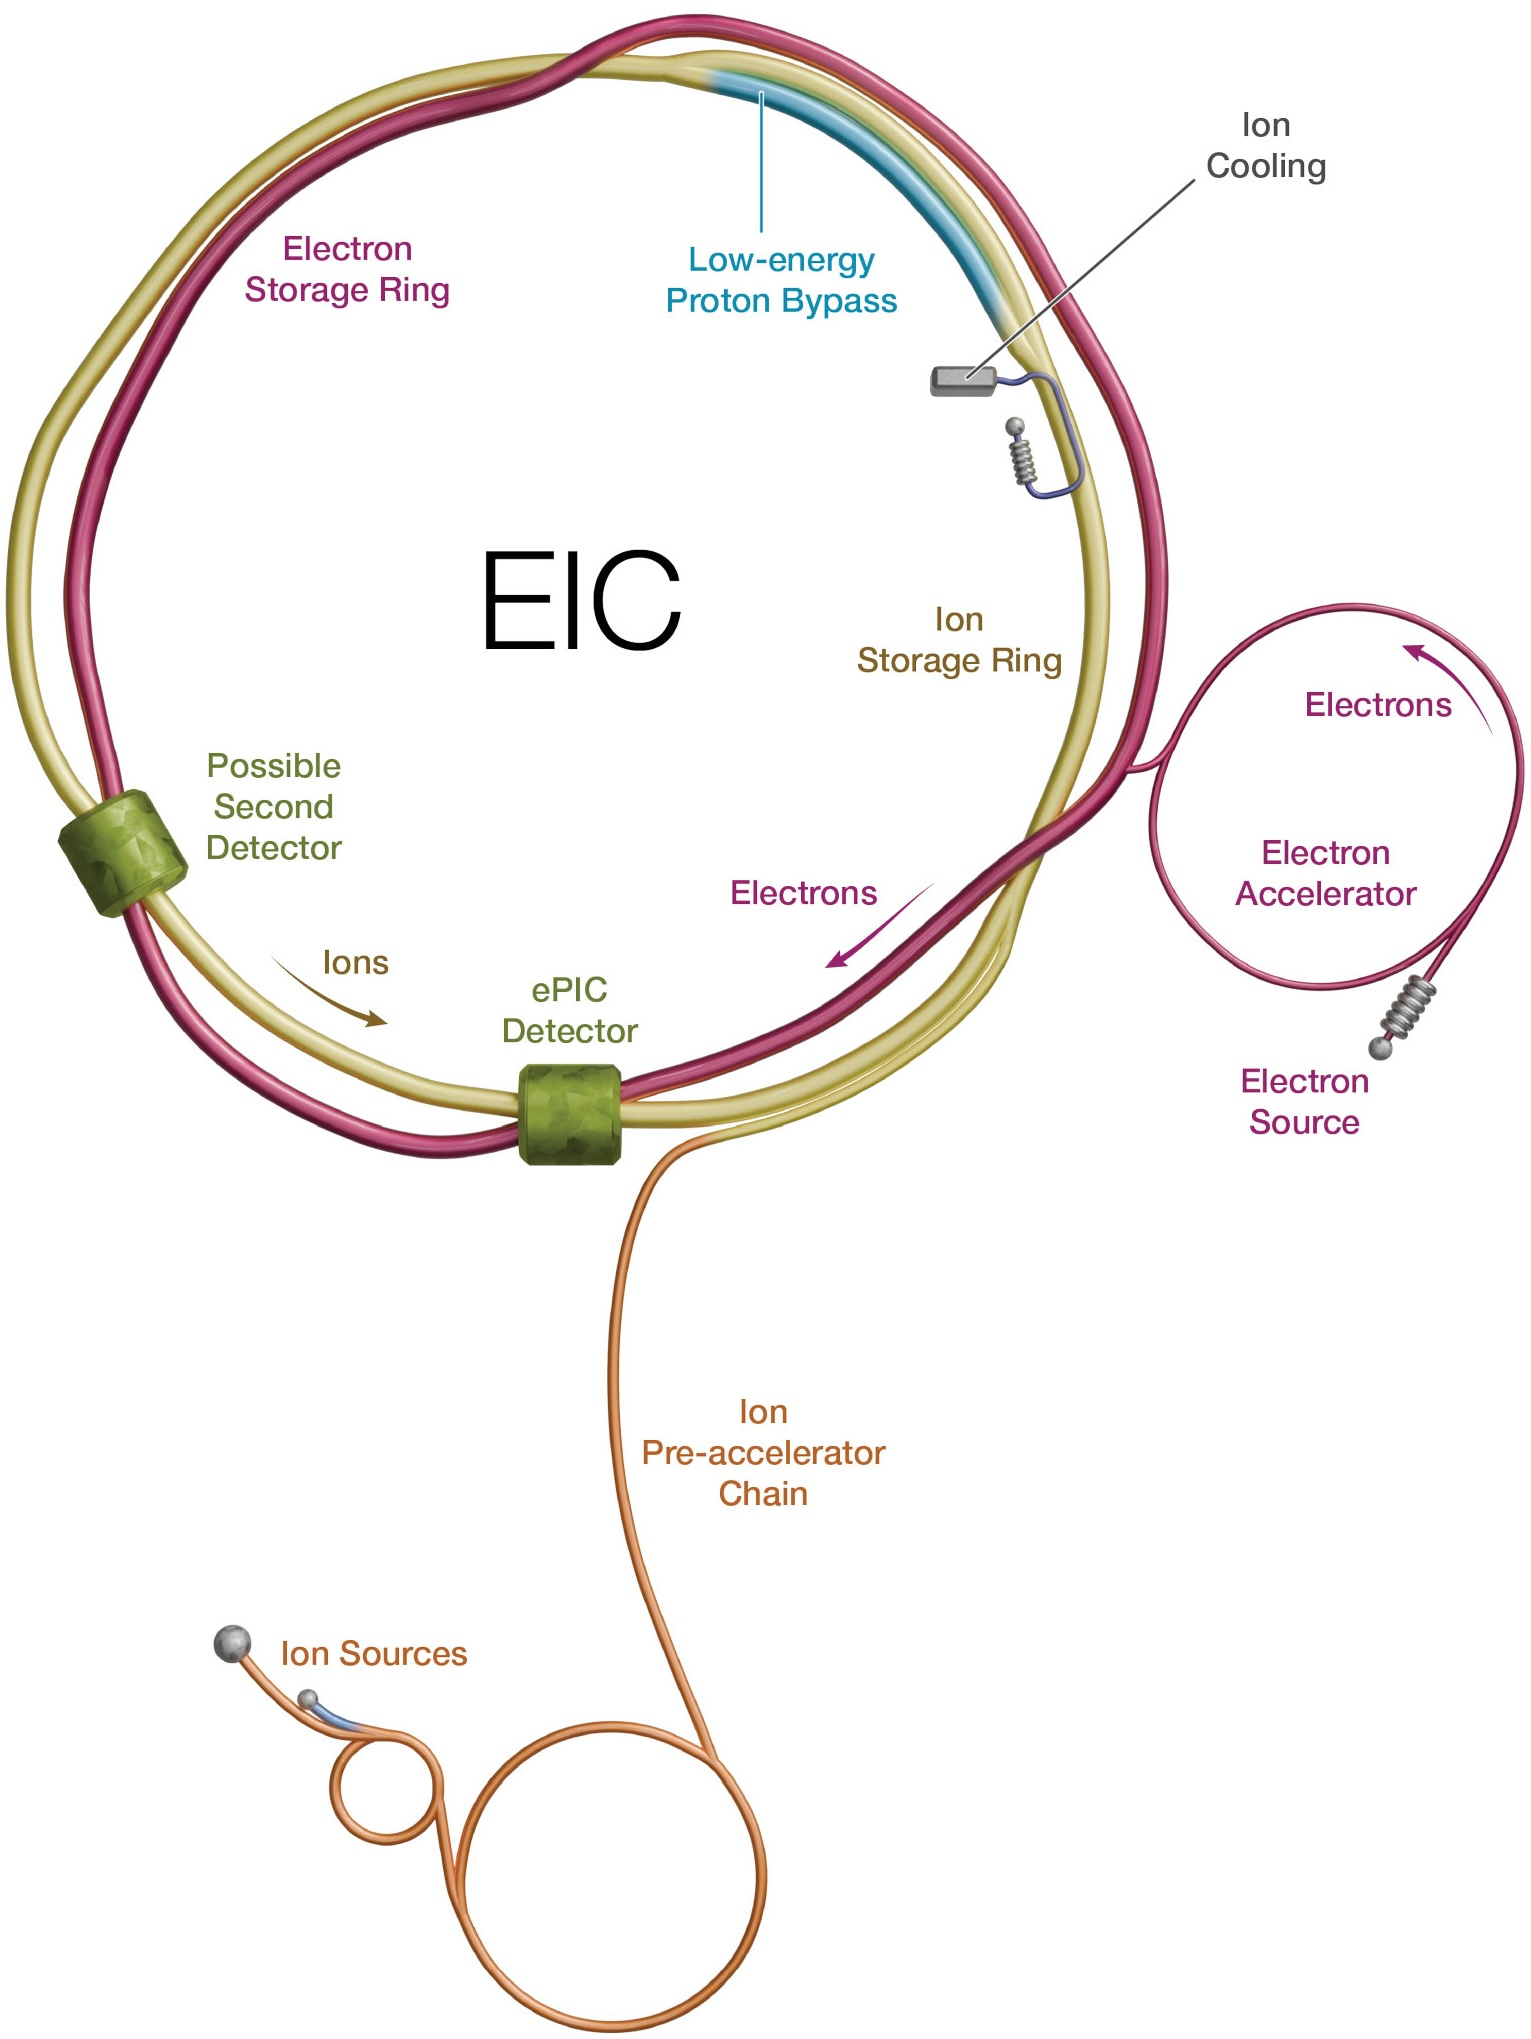
\includegraphics[width=.5\linewidth]{img/eic.jpg}
    \caption{\url{https://www.flickr.com/photos/brookhavenlab/54007751967/in/album-72157714316624996}}
    \label{fig:eic:eic}
\end{figure}

\begin{figure}[H]
    \centering
    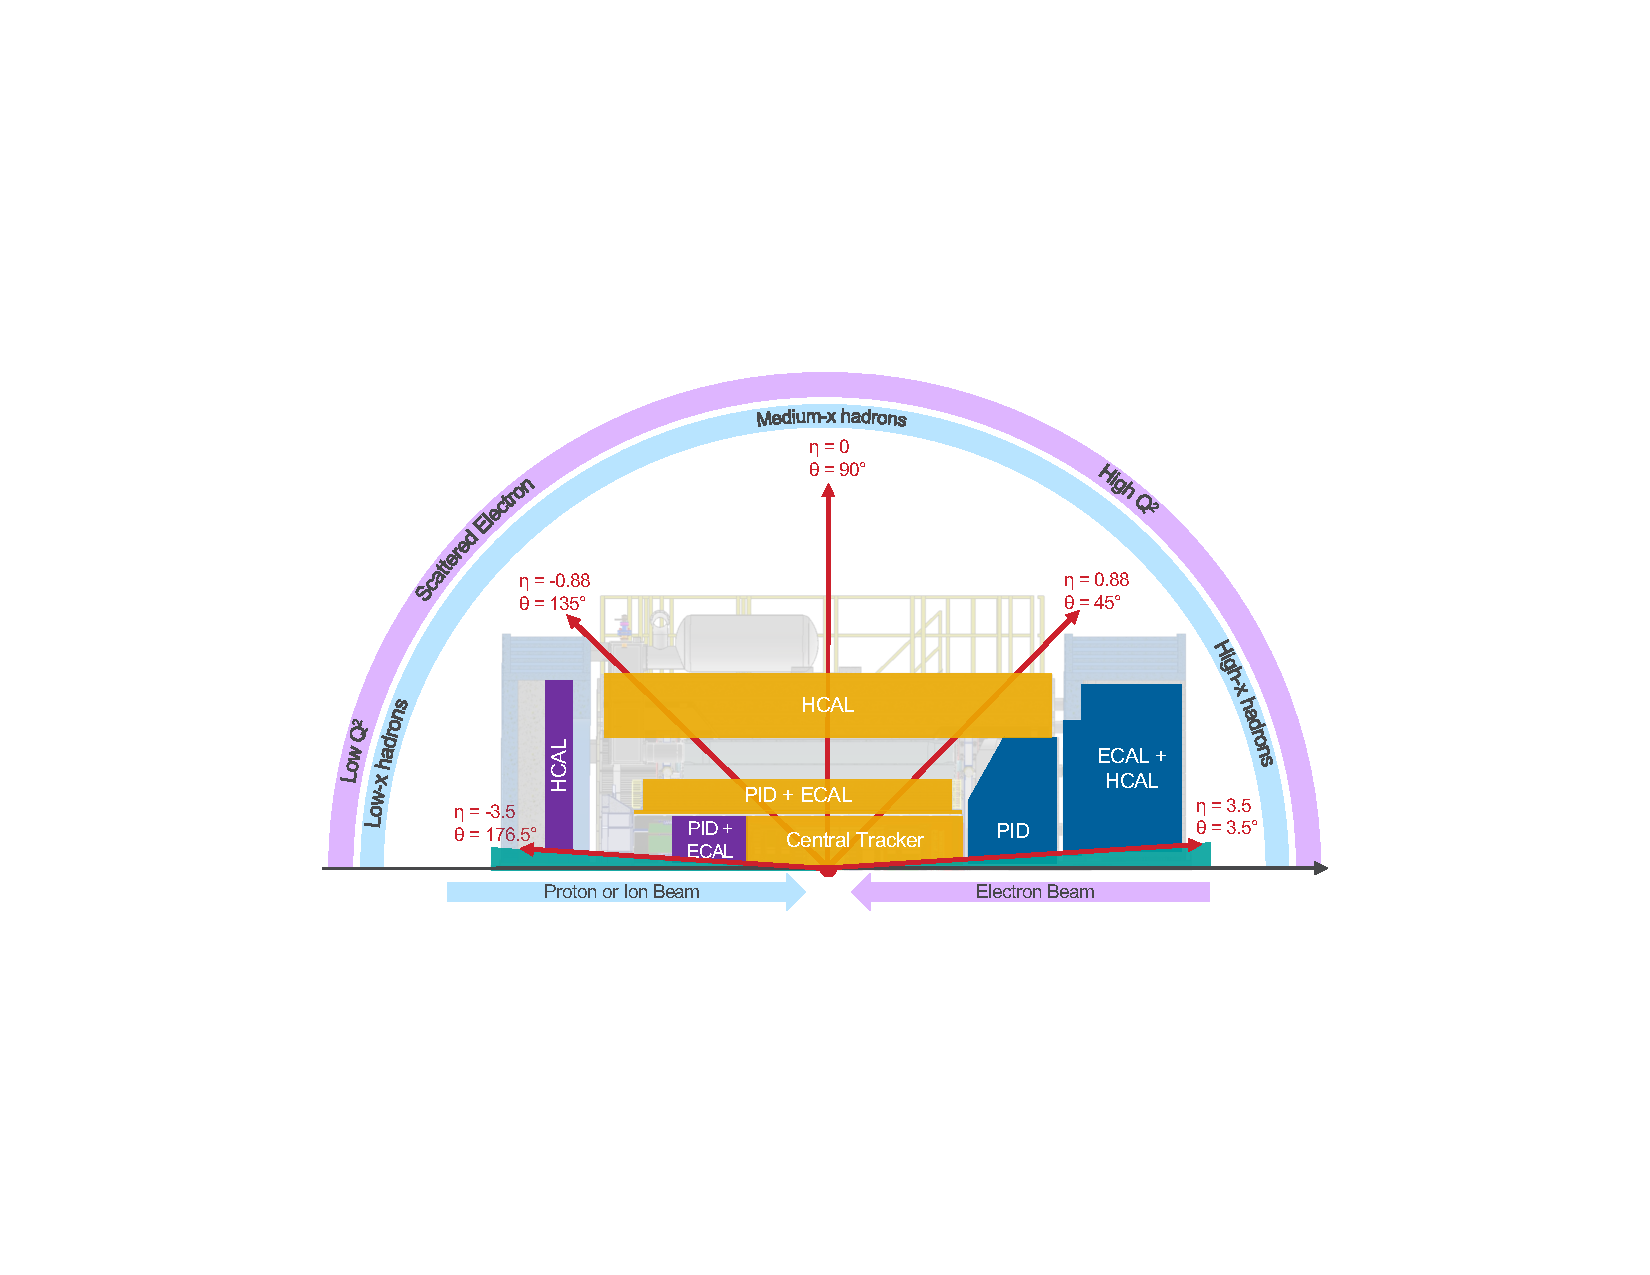
\includegraphics[width=.8\linewidth]{img/range.pdf}
    \caption{always this image \url{https://doi.org/10.5281/zenodo.14939545}}
    \label{fig:eic:range}
\end{figure}
maybe will fit better in another chapter



\section{Advantages? \textit{Prínosy}}